% \iffalse meta-comment
%  This file should be thesis.dtx
%
%%%%%%%%%%%%%%%%%%%%%%%%%%%%%%%%%%%%%%%%%%%%%%%%%%%%%%%%%%%%%%%%%%
%%                                                               %
%%    Thesis and Thesis Document Class for LaTeX2e               %
%%    South Dakota School of Mines and Technology                %
%%    By Larry Pyeatt                                            %
%%    Updated January 2017                                       %
%%    Written in May 2013                                        %
%%                                                               %
%%    Based on the Texas Tech University                         %
%%    Thesis and Thesis Document Class for LaTeX2e               %
%%    by Larry Pyeatt       May 2010                             %
%%                                                               %
%%    Based on the LaTeX2.09 style for Colorado State University %
%%    created by                                                 %
%%     Thad Mauney     Fall l984                                 %
%%     Revised Summer 1985 - Scott Douglas                       %
%%     Greatly revised June 1985 - Gary Herron                   %
%%     Customized for me, by me Jun'85 - P. Fitzhorn             %
%%     Customized more and better Dec'85 - Gary Herron, Tom Wood %
%%     Re-written for LaTeX2e and fixed Aug 1997- Larry Pyeatt   %
%%     Modified May, 2017 by Larry Pyeatt:                       %
%%       1. "Table of Contents" entry added to Table of          %
%%          Contents.                                            %
%%       2. Completely re-wrote the way appendices are handled.  %
%%       3. Updated documentation.                               %
%%       4. Changed default bibliography style to ieeetr.        %
%%                                                               %
%%                                                               %
%%%%%    NOT GUARANTEED TO PASS GRADUATE SCHOOL STANDARDS    %%%%%
%%        BUT CLOSE ENOUGH NOT TO BE A WASTE OF TIME             %
%%%%%%%%%%%%%%%%%%%%%%%%%%%%%%%%%%%%%%%%%%%%%%%%%%%%%%%%%%%%%%%%%%
%
%  This file is distributed in doctex format and contains both
%  documentation and macros in one file.  You need to generate
%  the documentation and the class file as follows:
%
%  STEP 1 - save the dtx file
%    Save this file as ``thesis.dtx''
%  STEP 2 - generate documentation
%    Type ``latex thesis.dtx'' to create thesis.dvi
%    You can print thesis.dvi or view it to see how
%    the thesis class works.
%  STEP 3 - generate the class file
%    1. Create a new file ``thesis.drv'' that contains:
%
%       \input docstrip
%       \generateFile{thesis.cls}{t}{\from{thesis.dtx}{class}}
%       \end
%       
%       If you cut and paste from here, don't forget to delete the `%' 
%       characters at the beginning of each line.
%
%    2. Type ``latex thesis.drv'' to  create the .cls file. 
%
%%%%%%%%%%%%%%%%%%%%%%%%%%%%%%%%%%%%%%%%%%%%%%%%%%%%%%%%%%%%%%%%%%
% \fi
% \iffalse
%%
%% File `thesis.dtx'.
%% Copyright (C) 2017 by Larry Pyeatt
% \fi
% \iffalse
%<*driver>
\documentclass{ltxdoc}
\textwidth 5.5in
\textheight 8.5in
\evensidemargin 1in
\oddsidemargin 1in
\headsep 0in
\topmargin 0in
\headheight 0in
\parindent 0in
\usepackage{xspace}
\begin{document}
\OnlyDescription
\DocInput{thesis.dtx}
%\input docstrip
%\generateFile{thesis.cls}{t}{\from{thesis.dtx}{class}}
%\end
\end{document}
%</driver>
% \fi
% \iffalse
%<class>\NeedsTeXFormat{LaTeX2e}
%<class>\ProvidesClass{thesis}[2013/05/20 South Dakota School of Mines and Technology Thesis and Dissertation Class]
%<class>\DeclareOption{twocolumn}{\OptionNotUsed}
%<class>\DeclareOption{titlepage}{\OptionNotUsed}
%<class>\DeclareOption*{\PassOptionsToClass{\CurrentOption}{report}}
%<class>\ProcessOptions\relax
%<class>\LoadClass{report}
%<class>\RequirePackage{ifthen}
%<class>\RequirePackage[pagestyles]{titlesec}
%<class>\RequirePackage{caption}
%%<class>\DeclareCaptionFont{xipt}{\fontsize{11}{13}\mdseries}
%%<class>\RequirePackage[font=xipt,labelfont=bf]{caption}
%%<class>\DeclareCaptionFont{xpt}{\fontsize{10}{12}\mdseries}
%%<class>\RequirePackage[font=xpt,labelfont=bf]{caption}
%<class>\DeclareCaptionFont{xvpt}{\fontsize{10.5}{12.5}\mdseries}
%<class>\RequirePackage[font=xvpt,labelfont=bf]{caption}
%<class>\RequirePackage{enumitem}
\newcommand{\schoolname}{South Dakota School of Mines and Technology\\Rapid City, South Dakota}
\newif\ifthesiscitations
\thesiscitationsfalse
\flushbottom
\newcommand{\drheading}{
\renewpagestyle{plain}{\sethead[\usepage][][]{}{DRAFT \today}{\usepage}}
}
% \fi
%
%
%\title{Disseration and Thesis Document Class}
%\author{Larry D. Pyeatt}
%\maketitle
% \section{Document Class}
% Your main file should have |\documentclass[12pt]{thesis}| as the
% first line.  This document class is based on the |report| class, so
% any option available in the |report| class should be available, with
% two exceptions: the |twocolumn| and |titlepage| options are not
% available in the thesis class.  For example
% |\documentclass[11pt,twocolumn]{thesis}| will not work.
% You should be
% able to use any package that works for the report document class.
% For example, |\usepackage{graphicx}| should work.
% \vspace{\baselineskip}
%
% The thesis class also includes an optional bibliography style and
% set of macros for doing citations similar to the way they are
% specified in the Chicago manual of style.  The bibliography style
% and citation package are based on the standard \LaTeX\xspace chicago
% bibliograhpy style and package.  \DescribeMacro{\bibliographystyle}
% You can use |\bibliographystyle{thesis}| if you have the
% |thesis.bst| file.  In that case, you should also use
% |\usepackage{thesiscitations}| to get the matching citation macros.
% There is a separate PDF file describing those extended |\cite|
% macros.
% \vspace{\baselineskip}
%
% If you are doing a Computer Science Thesis, then you should use
% |\bibliographystyle{acm}| or |\bibliographystyle{ieeetr}|, and
% \emph{not} have the |\usepackage{thesiscitations}| command.
%
% \section{Chapter Title Position}
%
% After the |\documentclass{}| statement, you can use one of these
% three commands to change the position of the chapter titles.  Chapter
% titles will be left justified unless you specify otherwise.
%
% \DescribeMacro{\lefttitles} The  |\lefttitles|
% command sets chapter titles to be left justified.
% \iffalse
\newcommand{\lefttitles}{
\def\ch@just{\raggedright}
}
\lefttitles
% \fi
%
% \DescribeMacro{\centertitles} The  |\centertitles|
% command sets chapter titles to be centered.
% \iffalse
\newcommand{\centertitles}{
\def\ch@just{\centering}
}
% \fi
%
% \DescribeMacro{\righttitles} The  |\righttitles|
% command sets chapter titles to be right justified.
% \iffalse
\newcommand{\righttitles}{
  \def\ch@just{\raggedleft}
}
% \fi
%
% \section{Optional Draft Commands}
% You can optionally specify the draft mode and spacing.  These
% commands allow you to print draft copies with single and 1.5 spacing
% to save paper. A doublespace draft mode is also available so you
% can check the final formatting.  If you do not
% specify a draft mode, then a final copy will be generated.
%
% \DescribeMacro{\ssdraft} shifts to single spacing and puts DRAFT
% in the heading of every page.
% \iffalse
\newcommand{\ssdraft}{
\setboolean{finalversion}{false}
\renewcommand{\doublespace}{\@normalsize\baselineskip\normalbaselineskip}
\drheading}
% \fi
%
% \DescribeMacro{\hsdraft} shifts to 1.5 spacing and puts DRAFT
% in the heading of every page.
% \iffalse
\newcommand{\hsdraft}{
\setboolean{finalversion}{false}
\renewcommand{\doublespace}{\@normalsize\baselineskip 1.45\normalbaselineskip}
\drheading}
% \fi
%
% \DescribeMacro{\dsdraft} shifts to double spacing and puts DRAFT
% in the heading of every page.  This mode should create a document
% that is identical to your final copy except for the DRAFT heading.
% \iffalse
\newcommand{\dsdraft}{
\setboolean{finalversion}{false}
\renewcommand{\doublespace}{\@normalsize\baselineskip 1.65\normalbaselineskip}
\drheading}
% \fi
%
% \section{Definitions}
%
% After the optional |\ssdraft|, |\hsdraft|, or |\dsdraft| statement, 
% you have to define some
% information that will be used for the cover sheet, running header, etc. 
% each of the following macros takes one argument.
%
% \DescribeMacro{\doctype}  defines the type of document and should
% be written as either
% |\doctype{thesis}| or |\doctype{dissertation}|.
% \iffalse
\newcommand{\doctype}[1]{\gdef\Zdoctype{#1}}
\doctype{---}
% \fi
%
% \DescribeMacro{\title} works just like in any other \LaTeX\xspace document.
% \iffalse
\renewcommand{\title}[1]{\gdef\Ztitle{#1}}
\title{---}
% \fi
%
% \DescribeMacro{\author} works just like in any other \LaTeX\xspace document.
% \iffalse
\renewcommand{\author}[1]{\gdef\Zauthor{#1}}
\author{---}
% \fi
%
% \DescribeMacro{\degree} defines the type of degree.  It should be\\
% |\degree{Doctor of Philosophy in Underwater Basket Weaving}|\\
% |\degree{Master of Science in Applied Handball}|\\
% |\degree{Master of Arts in Finger Painting}|\\ or whatever is
% appropriate for your degree.
% \iffalse
\newcommand{\degree}[1]{\gdef\Zdegree{#1}}
\degree{---}
% \fi
%
% \DescribeMacro{\defensedate} defines the date of the oral defense.
% For example:\\
% |\defensedate{January 12, 1988}|
% \iffalse
\newcommand{\defensedate}[1]{\gdef\Zdefdate{#1}}
\defensedate{---}
%\fi
%
% \DescribeMacro{\gradyear} defines the year you are graduating, It should be 
% four digits.
% \iffalse
\newcommand{\gradyear}[1]{\gdef\Zyear{#1}}
\gradyear{---}
% \fi
%
% \DescribeMacro{\department} defines the department that is granting
% your degree, examples:\\
% |\department{Department of Mathematics and Computer Science}|\\
% |\department{Department of Zoology}|\\
% |\department{Department of Redundancy Department}|
% \iffalse
\newcommand{\department}[1]{\gdef\Zdepartment{#1}}
\department{---}
% \fi
%
% \DescribeMacro{\signatureline} adds a line to the signature page where someone needs to sign. Examples:\\
% |\signatureline{Major Professor --- Dimm Whitt, Ph.D., Department of Zoology}|\\
% |\signatureline{Graduate Division Representative --- E.\ Nigma, Ph.D., Department of Philosophy}|\\
% |\signatureline{Committee Member --- Chip Munk, Ph.D., Department of Zoology}|\\
% |\signatureline{Head of the Zoology Department --- Earl E. Bird, Ph.D.}|\\
% |\signatureline{Dean of Graduate Education --- Raney Daze}|\\
%
% \iffalse
\newcommand{\make@signatureline}[1]{{%\footnotesize
\noindent\parbox{\textwidth}{\noindent\parbox[t][2\baselineskip]{4in}{\noindent\rule{4in}{1pt}\\\raggedright\noindent #1}\hfill\noindent\parbox[t]{1.5in}{\rule{1.5in}{1pt}\\\noindent Date}}}}
\newcommand{\make@signatures}{{\footnotesize\enlargethispage{\baselineskip}}%
}
\newcommand{\signatureline}[1]{\g@addto@macro\make@signatures{\par\vfill\noindent\make@signatureline{#1}}}
% \fi
%
% \section{Sections within the document}
% The thesis or dissertation is divided into 3 main sections: preliminaries, body, 
% and supplementaries.  There are 3 commands used to switch from one
% main section to the next.
%
% \DescribeMacro{\preliminaries} The preliminaries section is for maketitle,
% table of contents, etc and comes directly after the 
% the |\begin{document}| command.  
% \iffalse
\newcommand{\preliminaries}{\doublespace\pagestyle{plain}\eject
  \pagenumbering{roman}\setcounter{page}{1}}
% \fi
%
% \DescribeMacro{\body} The body section is for the main body of your work and
% it should come directly after the last section in the preliminaries. 
% \iffalse
\newcommand{\body}{\doublespace\vfill\pagebreak\eject
  \pagenumbering{arabic}\setcounter{page}{1}\eject}
% \fi
%
% \DescribeMacro{\supplementaries} The supplementary section contains the  
% bibliography, appendices, glossary, index, and vita.  
% \iffalse
\newcommand{\supplementaries}{\renewcommand{\@chapapp}{Appendix}
\setcounter{chapter}{0}\renewcommand{\thechapter}{\Alph{chapter}}}
% \fi
%
%\section{Commands and Environments in the Preliminaries}
% There are several commands and environments for use within the 
% preliminaries section.  
%
%\DescribeMacro{\maketitle}  The |\maketitle|
% command creates the title page, just as it does for other \LaTeX\xspace classes.
% \iffalse
\renewcommand{\maketitle}{%
\null%
\singlespace%
\pagestyle{empty}%
\thispagestyle{empty}%
\vspace{-2\baselineskip}%
\begin{center}%
{{\fontsize{14pt}{18pt}\selectfont
\bf\parbox{\textwidth}{\begin{center}\Ztitle\end{center}}}}\\%
{%\large
%\vspace{0.75\baselineskip}%
by\\%
\Zauthor\\%
\vspace{0.75\baselineskip}%
A \Zdoctype\ submitted to the Graduate Division\\%
in partial fulfillment of the requirements for the degree of\\%
\vspace{0.75\baselineskip}%
\Zdegree\\%
\vspace{0.75\baselineskip}%
\schoolname\\%
\vspace{0.75\baselineskip}%
Date Defended: \Zdefdate\\%
}\end{center}%
%% \vspace{\baselineskip}%
%% \noindent\parbox{\textwidth}{Prepared by:}%
%% \vfill%
%% \make@signatureline{\Zauthor}%
%% \par%
%% \vspace*{\baselineskip}%
\noindent\parbox{\textwidth}{Approved by:}%
\vfill%
\vspace*{-\baselineskip}%
\make@signatures%
}
\renewcommand\section{\@startsection{section}{1}{\z@}%
{-2.5ex \@plus -1ex \@minus -.2ex}%
{0.8ex \@plus.2ex}%
{\normalfont\large\bfseries}}                                   
\renewcommand\subsection{\@startsection{subsection}{2}{\z@}%
{-2.25ex\@plus -1ex \@minus -.2ex}%
{0.8ex \@plus .2ex}%
{\normalfont\normalsize\bfseries}}
\renewcommand\subsubsection{\@startsection{subsubsection}{3}{\z@}%
{-2.25ex\@plus -1ex \@minus -.2ex}%
{0.8ex \@plus .2ex}%
{\normalfont\normalsize\bfseries}}
\renewcommand\paragraph{\@startsection{paragraph}{4}{\z@}%
{2.25ex \@plus 1ex \@minus .2ex}%
{-1em}%
{\normalfont\normalsize\bfseries}}
\renewcommand\subparagraph{\@startsection{subparagraph}{5}{\parindent}%
{2.25ex \@plus 1ex \@minus .2ex}%
{-1em}%
{\normalfont\normalsize\bfseries}}
% \fi
%
% \DescribeMacro{\makecopyright} The  |\makecopyright|
% command creates a copyright page. Read the section
% about copyright in the Thesis and Dissertation Writing
% Instructions from the graduate school.
% \iffalse
\newcommand{\makecopyright}{\newpage\thispagestyle{empty}
\vspace*{0.3\textheight}%
\begin{center}%
  Copyright \copyright\ \Zyear, \Zauthor\\%
  All Rights Reserved%
\end{center}%
\vfill\vfill%
\newpage\doublespace}%
\def\@makeschapterhead#1{\newpage%
%\vspace*{-40\p@}%
{\parindent \z@ \ch@just%
\normalfont%
\interlinepenalty\@M%
\Large
\bfseries  #1\par\nobreak%
\vskip 40\p@
}}
\def\@makechapterhead#1{%
  {\parindent \z@ \ch@just \normalfont
  %{\centering\normalfont
    \ifnum \c@secnumdepth >\m@ne
    \Large
    \bfseries \@chapapp\space \thechapter
    \par\nobreak
    \vskip 20\p@
    \fi
    \interlinepenalty\@M
    \Large
    \bfseries #1\par\nobreak
    \vskip 40\p@
  }}
\def\@makeappendixhead#1{%
  {\parindent \z@ \ch@just \normalfont
  %%{\centering\normalfont
    \ifnum \c@secnumdepth >\m@ne
    \Large
    \bfseries Appendices
    \par\nobreak
    \vskip 20\p@
    \fi
    \interlinepenalty\@M
    \Large
    \bfseries #1\par\nobreak
    \vskip 40\p@
  }}
% \fi
%
% \DescribeEnv{abstract} The abstract environment is used
% the same as for any other \LaTeX\xspace document.  Just use
% |\begin{abstract} text \end{abstract}| as usual.
% \iffalse
%%\renewenvironment{abstract}{\singlespace\newpage
\renewenvironment{abstract}{\newpage
%%  \addcontentsline{toc}{chapter}{\protect\numberline{}Abstract}
  \addcontentsline{toc}{chapter}{Abstract}
  \@makeschapterhead{\centerline{Abstract}}
  \vskip 20pt\par\singlespace}{\newpage}%
%% This version prints the thesis/dissertation title
%% \renewenvironment{abstract}{\singlespace
%%   \addcontentsline{toc}{chapter}{Abstract}
%%   \@makeschapterhead{\centerline{Abstract}}
%%   \vskip 20pt\par\noindent Title: \Ztitle\par
%%   \vskip 0.5\baselineskip\strut\\%
%%   \noindent}{\newpage}%
% \fi
%
% \DescribeEnv{acknowledgments} The acknowledgments environment 
% creates a new page with at title for acknowledgments.  It
% works very much like the |abstract| environment.
% \iffalse
%% \newenvironment{acknowledgments}{\singlespace\newpage
\newenvironment{acknowledgments}{\newpage
%%  \addcontentsline{toc}{chapter}{\protect\numberline{}Acknowledgments}
  \addcontentsline{toc}{chapter}{Acknowledgments}
  \@makeschapterhead{\centerline{Acknowledgments}}
  \vskip 20pt\par}{\newpage}
% \fi
%
% \DescribeMacro{\tableofcontents}  The |\tableofcontents|
% macro makes a new page with the table of contents on it.
% It works just like it does in other document classes
% \iffalse
\def\contentsname{Table of Contents}
\renewcommand{\tableofcontents}{\singlespace\newpage
  \addcontentsline{toc}{chapter}{Table of Contents}
  \@makeschapterhead{\centerline{Table of Contents}}
  \vskip 20pt\par\@starttoc{toc}}
% \fi
%
% \DescribeMacro{\listoftables} The |\listoftables| macro makes a new
% page with the list of tables on it.  It works just like it does in
% other document classes
% \iffalse
\renewcommand{\listoftables}{\singlespace\newpage
\addcontentsline{toc}{chapter}{List of Tables}
%%\addcontentsline{toc}{chapter}{\protect\numberline{}List of Tables}
  \@makeschapterhead{\centerline{List of Tables}}
  \vskip20pt
  \@starttoc{lot}}
% \fi
%
% \DescribeMacro{\listoffigures} The |\listoffigures| macro makes a
% new page with the list of figures on it.  It works just like it does
% in other document classes
% \iffalse
\renewcommand{\listoffigures}{\singlespace\newpage
  \addcontentsline{toc}{chapter}{List of Figures}
%%  \addcontentsline{toc}{chapter}{\protect\numberline{}List of Figures}
  \@makeschapterhead{\centerline{List of Figures}}
  \vskip20pt
  \@starttoc{lof}}
% \fi
%
% \DescribeEnv{listofsymbols} The |listofsymbols| environment lets you
% include a table of symbols and acronyms.  You must build the table
% yourself within the environment, using the table or other environments.
% Use |\begin{listofsympols}| text 
% |\end{listofsymols}| if you want one.
% \iffalse
\newenvironment{listofsymbols}{\singlespace\newpage
%%  \addcontentsline{toc}{chapter}{\protect\numberline{}List of Symbols and Acronyms}
  \addcontentsline{toc}{chapter}{List of Symbols and Acronyms}
  \@makeschapterhead{\centerline{List of Symbols and Acronyms}}
  \vskip 20pt\par}{\newpage}
% \fi
%
% \DescribeEnv{listofkeywords} The |listofkeywords| environment lets
% you include a table of keywords.  You must build the table yourself
% within the environment.  Use |\begin{listofkeywords}| |text|
% |\end{listofkeywords}| if you want one.
% \iffalse
\newenvironment{listofkeywords}{\singlespace\newpage
%%  \addcontentsline{toc}{chapter}{\protect\numberline{}List of Keywords}
  \addcontentsline{toc}{chapter}{List of Keywords}
  \@makeschapterhead{\centerline{List of Keywords}}
  \vskip 20pt\par}{\newpage}
% \fi
%
% \DescribeEnv{dedication} The dedication environment 
% creates a new page with at title for the dedication.  It
% works very much like the |abstract| environment.
% \iffalse
%%\newenvironment{dedication}{\singlespace\newpage
\newenvironment{dedication}{\newpage
%%  \addcontentsline{toc}{chapter}{\protect\numberline{}Dedication}
  \addcontentsline{toc}{chapter}{Dedication}
  \@makeschapterhead{\centerline{Dedication}}
  \vskip 20pt\par}{\newpage}
% \fi
%
% \DescribeEnv{preface} The preface environment 
% creates a new page with at title for the preface.  It
% works very much like the |abstract| environment.
% \iffalse
%%\newenvironment{preface}{\singlespace\newpage
\newenvironment{preface}{\newpage
  %%  \addcontentsline{toc}{chapter}{\protect\numberline{}Preface}
  \addcontentsline{toc}{chapter}{Preface}
  \@makeschapterhead{\centerline{Preface}}
  \vskip 20pt\par}{\newpage}
% \fi
%
% \section{Commands and environments within the body}
% Commands and envionments within the body text should work as normal
% for the report document class.  Use |\chapter{}|, |\section{}|, etc.
% You may wish to write the body in a separate file and just include 
% it at the appropriate place.
%
% \section{Commands and environments within the supplementaries}
% The supplementaries section contains the bibliography, appendices, 
% and other additional information that you may wish to include.
% There is a file named |thesis.bst| that is supposed to
% be supplied with the thesis class.
% If you do not have |thesis.bst|, or do not want to use it, then you can use
% the Chicago bibliography style (or any style appropriate for your field).
% Other than that, the bibliography should be created as you would
% for any other document class. 
%
% \iffalse
\renewcommand{\thebibliography}[1]{
 \@makeschapterhead{\centerline{Bibliography}}
 \vskip20pt
%% \addcontentsline{toc}{chapter}{\protect\numberline{}References}
 \addcontentsline{toc}{chapter}{Bibliography}
 \singlespace
 \list{[\arabic{enumi}]}{\settowidth\labelwidth{[#1]}
 \leftmargin\labelwidth 
 \advance\leftmargin\labelsep
   \advance\leftmargin\bibindent
   \itemindent -\bibindent
   \listparindent \itemindent
   \parsep \z@
 \usecounter{enumi}}
 \def\newblock{\hskip .11em plus .33em minus -.07em}
 \sloppy
 \sfcode `\.=1000\relax}
% \fi
%
% \DescribeEnv{appendices} The |appendices| environment is used to create
% the appendices.  Within this environment, the |\appendix| macro is used to
% create individual appendices.  The |\appendix| macro works just like the
% |\chapter| macro, but generates an appendix rather than a chapter.
% \iffalse
\newenvironment{appendices}{
\if@openright\cleardoublepage\else\clearpage\fi
 \addcontentsline{toc}{chapter}{Appendices}
 \thispagestyle{plain}\parindent\z@
 \parskip\z@ \@plus .3\p@\relax}
  {\clearpage}
% \fi
%
% \DescribeMacro{\appendix} The |\appendix| macro works like |\chapter|, but
% |\appendix| in used within the |appendix| environment.
% \iffalse
\renewcommand\appendix{\if@openright\cleardoublepage\else\clearpage\fi
                    \thispagestyle{plain}%
                    \global\@topnum\z@
                    \@afterindentfalse
                    \secdef\@appendix\@schapter}
\def\@appendix[#1]#2{\ifnum \c@secnumdepth >\m@ne
                         \refstepcounter{chapter}%
                         \typeout{\@chapapp\space\thechapter.}%
                         \addcontentsline{toc}{section}%
                         %%{\protect\numberline{Appendix \thechapter}}%
                         {Appendix \thechapter}%
                    \else
                    %% \addcontentsline{toc}{section}{#1}%
                    %% \addcontentsline{toc}{section}{}%
                    \fi
                    \chaptermark{#1}%
                    \addtocontents{lof}{\protect\addvspace{10\p@}}%
                    \addtocontents{lot}{\protect\addvspace{10\p@}}%
                    \if@twocolumn
                      \@topnewpage[\@makeappendixhead{#2}]%
                    \else
                      \@makeappendixhead{#2}%
                      \@afterheading
                    \fi}
% \fi
%
% \DescribeEnv{gloss} The |gloss| environment is used to create
% a glossary.  The environment starts a new page and puts an
% appropriate heading, you have to fill in the text yourself.
% Use |\begin{glossary}| |text| |\end{glossary}| to create a glossary.
% \iffalse
\newenvironment{gloss}{
 \newpage\@makeschapterhead{\centerline{Glossary of Terms}}
%% \addcontentsline{toc}{chapter}{\protect\numberline{}Glossary of Terms}
 \addcontentsline{toc}{chapter}{Glossary of Terms}
 \thispagestyle{plain}\parindent\z@
 \parskip\z@ \@plus .3\p@\relax}
 {\clearpage}
% \fi
%
% \DescribeEnv{abbreviations} The |abbreviations| environment is used to create
% list of abbreviations.  The environment starts a new page and puts an
% appropriate heading, you have to fill in the text yourself.
% Use |\begin{abbreviations}| |text| |\end{abbreviations}| to 
% create a list of abbreviations.
% \iffalse
\newenvironment{abbreviations}{
 \@makeschapterhead{\centerline{List of Abbreviations}}
 %% \addcontentsline{toc}{chapter}{\protect\numberline{}List of Abbreviations}
 \addcontentsline{toc}{chapter}{List of Abbreviations}
 \thispagestyle{plain}\parindent\z@
 \parskip\z@ \@plus .3\p@\relax}
 {\clearpage}
% \fi
%
% \DescribeMacro{\makeindex} The index generation macros work the same
% as in other document classes. Put |\usepackage{makeidx}| and
% |\makeindex| somewhere before
% |\begin{document}| if you want to use makeindex to create an index.
%
% \DescribeMacro{\index} Use the |\index| macro as described in
% ``The \LaTeX\xspace Companion'' and ``\LaTeX: a Document Preparation
%  Language'' to add entries to your index.
%
% \DescribeMacro{\printindex} The |\printindex| macro is used to insert
% an index created by the |makeindex| program.  
% The macro starts a new page and puts an
% appropriate heading, then inserts the index. 
% \iffalse
\def\indexname{Index}
\renewenvironment{theindex}{
% \newpage\singlespace
 \columnseprule \z@
 \columnsep 35\p@
 \twocolumn[\@makeschapterhead{\centerline{\indexname}}]%
%% \addcontentsline{toc}{chapter}{\protect\numberline{}Index}
 \addcontentsline{toc}{chapter}{Index}
 \thispagestyle{plain}\parindent\z@
 \parskip\z@ \@plus .3\p@\relax
 \let\item\@idxitem}
 {\onecolumn\clearpage}
% \fi
%
% \DescribeEnv{vita} The vita environment creates a new page with at
% title for the vita.  It works very much like the |abstract|
% environment. All SDSMT theses and dissertations must have a vita,
% not over one page in length.  It must be the last page in the thesis
% or dissertation and must contain the following information:
% \begin{enumerate}
% \item place and date of birth,
% \item place and date of high school graduation,
% \item place and date of college graduation, including degree an major,
% \item place and date of receipt of master's degree, including major, (for dissertations only), 
% \item vocational and professional experience (not summer jobs), including dates, nature of position, and school or organization,
% \item military experience, with indication of professional relevance, if any,
% \item scholarly publications, exhibits of creative work, membership in professional organizations and honorary societies.
% \end{enumerate}
% \iffalse
\newenvironment{vita}{\newpage
%%  \addcontentsline{toc}{chapter}{\protect\numberline{}Vita}
  \addcontentsline{toc}{chapter}{Vita}
  \@makeschapterhead{\centerline{Vita}}
  \vskip 20pt\par}{\newpage}
% \fi
%
% \section{General use commands and defaults}
% \DescribeMacro{\singlespace} The |\singlespace| command is used to 
% switch to single spacing mode, and 
% \DescribeMacro{\doublespace} 
% |\doublespace|is used to switch to double spacing mode.
%NOTE: The doublespace command is overridden by the |\ssdraft| and |\hsdraft|
% commands!
% \iffalse
\newcommand{\singlespace}{\@normalsize \baselineskip \normalbaselineskip}
\newcommand{\doublespace}{\@normalsize \baselineskip 1.65\normalbaselineskip}
% \fi
%
% \iffalse
\widowpenalty=10000
\clubpenalty=10000
%% I don't know why the margins have to be set like this.  Makes no sense.
\textwidth 6.25in
\evensidemargin 0.375in
\oddsidemargin 0.375in
%% \evensidemargin 0.5in
%% \oddsidemargin 0.5in
%% \textwidth 6in
\textheight 9in
\footskip\baselineskip
%\addtolength{\textheight}{-\footskip}
\topmargin 0in
\headheight \normalbaselineskip
\headsep 0.25in
\widenhead{0.25in}{0.25in}
\renewpagestyle{plain}{\sethead[\usepage][][]{}{}{\usepage}}
\pagestyle{plain}
\addtolength{\topmargin}{-\headheight}
\addtolength{\topmargin}{-\headsep}
\setcounter{secnumdepth}{5}
\setcounter{tocdepth}{5}
\footnotesep 1.65\baselineskip
\setlength{\skip\footins}{1.65\baselineskip}
\renewcommand{\footnoterule}{\noindent\vspace*{-3pt}\rule{1.5in}{0.4pt}\vspace*{2.6pt}}
\newboolean{finalversion}
\setboolean{finalversion}{true}
\renewcommand\l@chapter[2]{%
  \ifnum \c@tocdepth >\m@ne
  \addpenalty{-\@highpenalty}%
  \vskip 1.0em \@plus\p@
  \setlength\@tempdima{1.5em}%
  \begingroup
  \parindent \z@ \rightskip \@pnumwidth
  \parfillskip -\@pnumwidth
  \leavevmode \bfseries
  \advance\leftskip\@tempdima
  \hskip -\leftskip
  #1\nobreak\normalfont\leaders\hbox{$\m@th
    \mkern \@dotsep mu\hbox{.}\mkern \@dotsep
    mu$}\hfill\nobreak\hb@xt@\@pnumwidth{\hss #2}\par
  \penalty\@highpenalty
  \endgroup
  \fi}
\renewcommand*\l@section{\@dottedtocline{1}{1.5em}{2.3em}}
\renewcommand*\l@subsection{\@dottedtocline{2}{3.8em}{3.2em}}
\renewcommand*\l@subsubsection{\@dottedtocline{3}{7.0em}{4.1em}}
\renewcommand*\l@paragraph{\@dottedtocline{4}{10em}{5em}}
\renewcommand*\l@subparagraph{\@dottedtocline{5}{12em}{6em}}
% \fi
%
% \section{Example}
% \begin{verbatim}
% \documentclass[12pt]{thesis}

% \usepackage{graphicx}
% \usepackage{makeidx}
% \usepackage{subfig}

% % Uncomment the following two lines and comment out the third one
% % if you want to use the Chicago Manual based bibliography.
% %\usepackage{thesiscitations}
% %\bibliographystyle{thesis}
% \bibliographystyle{ieeetr}

% % Uncomment next line if you want chapter titles centered
% %\centertitles

% Uncomment next line to print a double-spaced draft version
% %\dsdraft

% Uncomment next line to print a single-spaced draft version
% %\ssdraft

% \makeindex

% \doctype{thesis}
% \title{A Compative Study of Gnus and Gnats}
% \author{Harvey Finklebaum}
% \degree{Doctor of Philosophy in Zoology}
% \defensedate{April 4, 2013}
% \gradyear{2013}
% \department{Zoology}

% % The following commands add a signature line for each person who needs
% % to sign the thesis/dissertation
% \signatureline{Major Professor --- Dimm Whitt, Ph.D., Department of Zoology}
% \signatureline{Graduate Division Representative --- E.\ Nigma, Ph.D., Department of Philosophy}
% \signatureline{Committee Member --- Chip Munk, Ph.D., Department of Zoology}
% \signatureline{Committee Member --- Gail Force, Ph.D., Department of Meteorology }
% % the line break in the next line makes the spacing come out right.
% \signatureline{Head of the Zoology Department ---   Earl E. Bird, Ph.D.\\}
% \signatureline{Dean of Graduate Education --- Raney Daze}

% \begin{document}
% \maketitle
% \preliminaries

% \begin{abstract}
% I present a fascinating and
% thought provoking study, comparing gnus and gnats.
% The results of the study show conclusively that there
% is no resemblance between the two, whatsoever.
% \end{abstract}

% \begin{acknowledgments}
% I would like to thank my advisor, Dr.\ Dimm Whitt, for
% all of the support he has given me.
% \end{acknowledgments}

% \tableofcontents

% \listoftables

% \listoffigures

% \begin{listofsymbols}
% \begin{tabular}{ll}
% $\mathcal{G}_t$ & Gnat\\
% $\mathcal{G}_u$ & Gnu
% \end{tabular}
% \end{listofsymbols}

% \begin{listofkeywords}
% \noindent Gnat, Gnu.
% \end{listofkeywords}

% \begin{dedication}
% In loving memory of 
% my grandmother.
% \end{dedication}

% \begin{preface}
% Before we begin, just let me say one thing.
% Gnat and gnu are both begin with ``gn,'' and
% the purpose of this work was to see if there
% are any other resemblances.
% This thesis has taken 45 years of work, and
% I don't have much time left in this world, but it
% has been worth it.  When the time comes,
% I would like to die as my grandmother did, peacefully in
% her sleep, not screaming like the passengers in her car.
% \end{preface}

% \body

% \chapter{Introduction}
% This thesis is the first work ever done in 
% the fascinating study of comparison of gnats to gnus.
% It is groundbreaking.  There literally is nothing
% like it.  However, there have been a few studies
% of other things.

% For example, \citeN{Kringle} showed that apples and
% goats have almost nothing in common, other than both
% being red.  The major problem with Kringle's study is that
% he used a goat that had been spray painted red, and 
% his apple was a golden delicious variety.  Criticism
% of Kringle's methods has been harsh, and so far, no
% one has been able to replicate his results.

% Several researchers have compared trout to eagles\cite{Simmons,Sheppard}.
% The consensus that has emerged is that they are quite different,
% and only an idiot would try to eat an eagle\cite{Idiot}.

% \chapter{Comparison}
% In this chapter, I will present the methods for my comparison, the
% results, and fill in with a lot of gibberish.  For instance, I will
% say things like ``Gnats and Gnus come in twos'' in order to fill space
% and make my thesis seem longer than it really is.  This is a tactic
% used by some people to hide the fact that their research is worthless.
% The idea is that if the thesis is long enough and boring enough, the
% thesis comittee members will go to sleep every time they try to read it.

% Another thing that I may do is to use very long words, such as
% onomatopoeia, for no apparent reason.  By employing voluminous
% instances of obfuscatory and expansive vocables, the lack of
% quintessence of this monograph can be adumbrated from all but
% the most erudite, didactic, and scholarly bibliophiles.

% \section{Visual comparison}
% \index{comparison!visual}

% \begin{table}
% \caption{Results of visual comparison studies.}
% \begin{center}
%   \begin{tabular}{|c|c|}
%     \hline
%     \bf Categories & \bf Percent Correct\\
%     \hline
%     \hline
%     insect/mammal & 76\\
%     \hline
%     gnat/gnu & 69\\
%     \hline
%   \end{tabular}
% \end{center}
% \label{table:comp1}
% \end{table}

% The first test that I performed was a visual comparison of gnats and
% gnus.  First, I went on the internet and downloaded several thousand
% pictures of gnats, and one picture of a gnu.  Then, I had two
% volunteers compare them and categorize them as insect\index{insect} or
% mammal.\index{mammal} Next, I selected another group of volunteers and
% had them classify the photographs as either gnat or gnu.


% The results of this comparison are shown in Table~\ref{table:comp1}.
% As can be seen, both volunteers (myself and my advisor) were able to
% correctly classify most of the photographs.  As a result, we gave each
% other little gold stars.  
% \begin{figure}
% \begin{center}
% \subfloat{\resizebox{2in}{!}{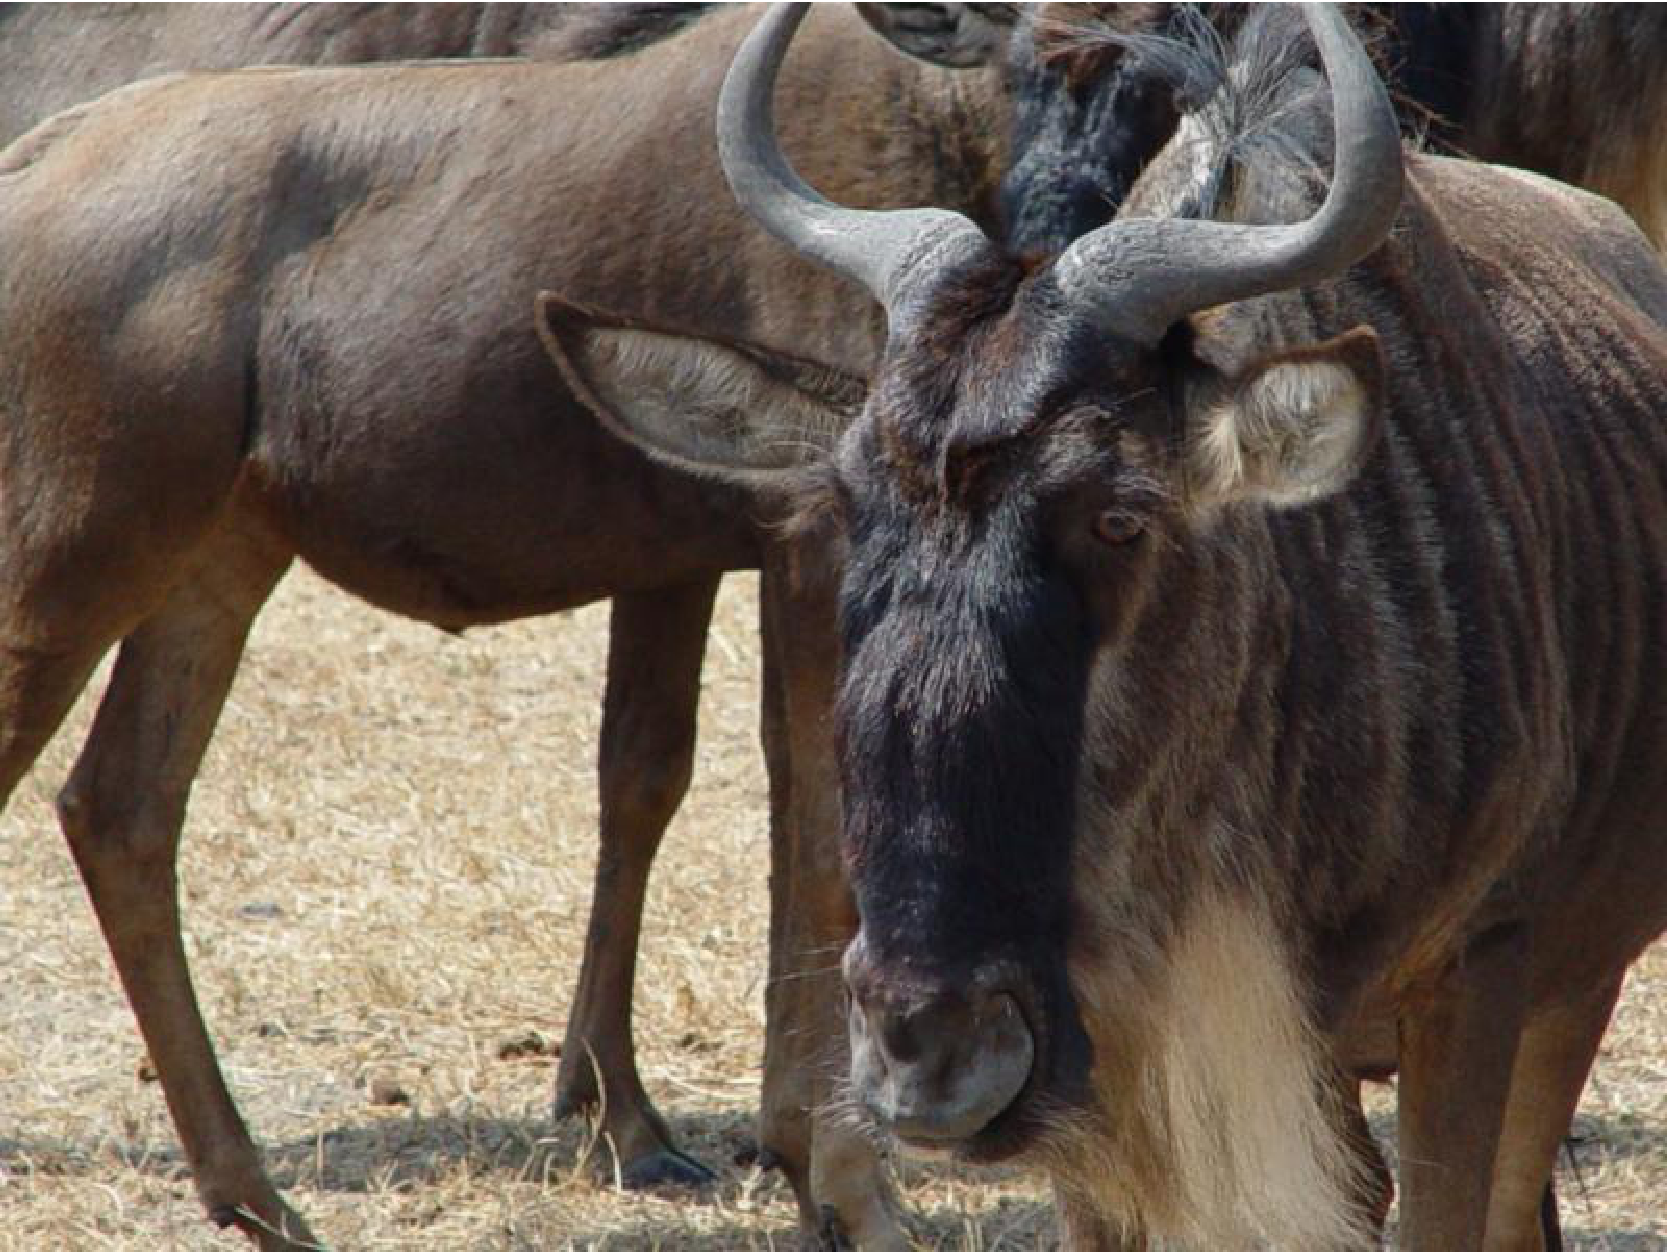
\includegraphics{images/gnu.pdf}}}
% \subfloat{\resizebox{2in}{!}{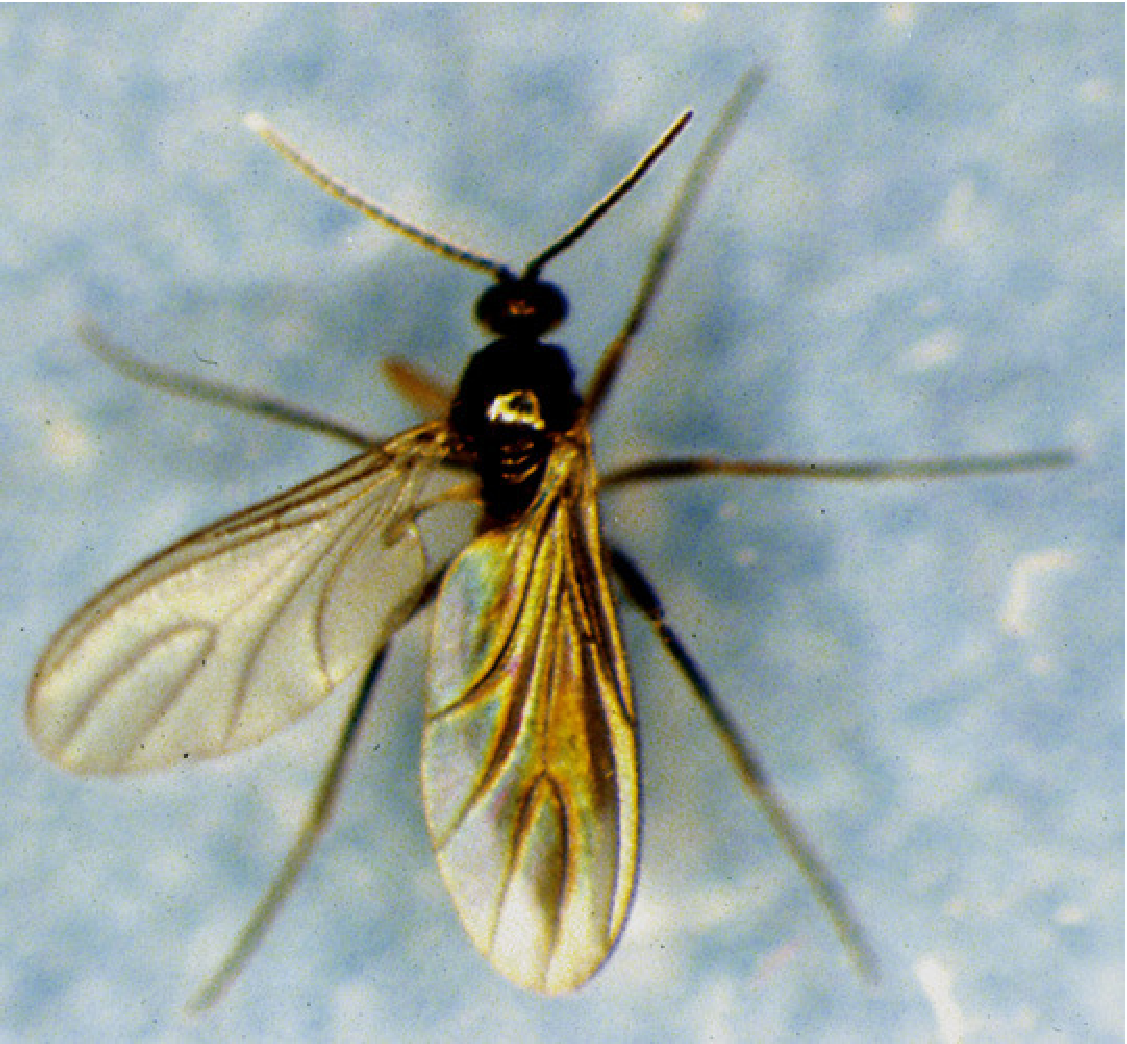
\includegraphics{images/gnat.pdf}}}
% \end{center}
% \caption{Photographs of a gnu (left) and a gnat (right).}
% \label{figure:photos}
% \end{figure}
% For those who are interested,
% Figure~\ref{figure:photos} shows the gnu photograph and one of the gnat
% photographs.

% \section{Comparison by Size}
% \index{comparison!size}
% As can be seen from Figure~\ref{figure:photos}, photographs of
% gnats are slightly larger than photographs of gnus.  This leads
% us to believe that statistically, gnats are slightly larger
% than gnus.  Mathematically, we express this as follows:
% \begin{equation}
% S(\mathcal{G}_t) > S(\mathcal{G}_u) \forall \mathcal{G}_t,\mathcal{G}_u,
% \end{equation}
% where $\mathcal{G}_t$ is a photograph of a gnat and
% $\mathcal{G}_u$ is a photograph of a gnu.  The $S()$ function
% calculates the ``size'' of the photograph.

% \chapter{Conclusions}

% Well, there you have it.  My advisor and I were able to
% tell the difference between a photograph of a gnat and
% a gnu most of the time.  Also, gnats are larger than gnus, and
% therefore, they are significantly different.

% In the future, we plan to apply the techniques developed
% in this research to answer the age old question of 
% whether dogs and ducks are the same thing.

% \supplementaries

% \pagebreak

% \bibliography{harvey.bib}

% \begin{appendices}

% \appendix{Appendix A} Well, I really have nothing more to say,
% but wanted to have an appendix.

% \end{appendices}

% \begin{gloss}
% I don't have a glossary either, but this is what the page
% would look like if I did.
% \end{gloss}

% %\begin{abbreviations}
% %gnu is abbreviated to gnu\\
% %gnat is abbreviated to gnat
% %\end{abbreviations}

% \printindex

% \begin{vita}
% \noindent Born: July 4, 1776, Cancun, Mexico.\\
% Education:
% High school: Napolean Bonaparte High, Versailles, 1923.
% College: Bachelor of Science in Basket Weaving, Harvard on the Hill, Paris, Texas, 1989.
% \end{vita}

% \end{document}

%\end{verbatim}
